\documentclass[conference]{IEEEtran}
\IEEEoverridecommandlockouts
% The preceding line is only needed to identify funding in the first footnote. If that is unneeded, please comment it out.
\usepackage{cite}
\usepackage{amsmath,amssymb,amsfonts}
\usepackage{algorithmic}
\usepackage{graphicx}
\usepackage{textcomp}
\usepackage{xcolor}
\def\BibTeX{{\rm B\kern-.05em{\sc i\kern-.025em b}\kern-.08em
    T\kern-.1667em\lower.7ex\hbox{E}\kern-.125emX}}
\begin{document}

\title{ADLR WS21 - Milestone Report Team 04\\
}

\author{\IEEEauthorblockN{Marc Hauck}
\IEEEauthorblockA{\textit{Robotics, Cognition, Intelligence} \\
\textit{Technical University of Munich}\\
Munich, Germany \\
ge65qoy@mytum.de}
\and
\IEEEauthorblockN{Baris Tura}
\IEEEauthorblockA{\textit{Robotics, Cognition, Intelligence} \\
\textit{Technical University of Munich}\\
Munich, Germany \\
baris.tura@tum.de}}

\maketitle

\section{Experiments}

\subsection{Discrete Environments}

To get familiar with the Stable-Baselines 3 (SB3) library and the environment inherited from the Open AI gym class, we started with an empty 10x10 grid world environment with no obstacles. The agent always started in the top left corner and had to find the goal in the bottom right corner by taking one of the actions UP, DOWN, RIGHT and LEFT. Similar to the approach in \cite{b1}, the reward was set to 1 at the goal and 0 else. Using a discrete observation and action space, the experiments needed only little computation time and the agent was able to overfit to this environment quickly. For all experiments so far, we used the reinforcement learning algorithm Proximal Policy Optimization (PPO), as it was suggested by the SB3 documentation.

In a second step, we added obstacles to the environment and initially rewarded a collision with -1. Adding the obstacles led to a massive increase of computation time as they increased the dimension of the observation space depending on the number of obstacles. Additionally, it required changes of the reward function: If the negative reward of a collision was too small compared to the reward for reaching the goal, the agent would ignore the obstacle and step over it. This was still possible because we did not reset the environment upon collision. If the negative reward for colliding was too high compared to the goal reward, the agent would not move at all and stay in its corner. After increasing the number of training steps and finding a good ratio between positive and negative rewards by using binary search, we were able to successfully train the agent in this environment.

\begin{figure}[htbp]
\centerline{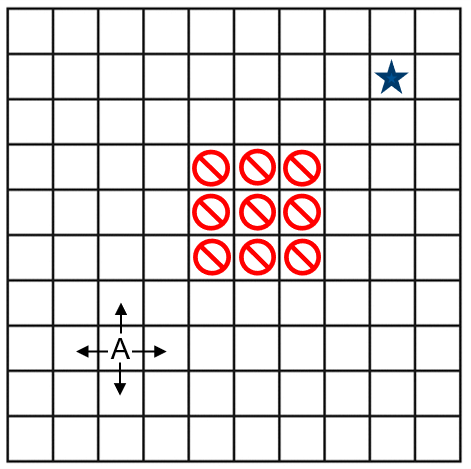
\includegraphics{discrete.png}}
\caption{10x10 discrete environment: The agent (A) has to find the goal (star) without clliding with the obstacles (do-not-cross signs).}
\label{fig1}
\end{figure}

\subsection{Continuous Environments}

Next, we transformed the environment to a continuous one in [0, 10] x [0, 10]. To enable the agent to freely move in the continuous space, the two-dimensional action space was initially set to [-1, 1] for the agent's velocity in x- and y-direction. The experiments started with the sparse rewards from the discrete environment and no obstacles, but the agent was not able to find the goal reliably. As long as the positions of start and goal were fixed, the agent was able to overfit to the goal's position and find it, but if we sampled start and goal position only from small intervals, the agent often walked past the goal and ended up stuck in a corner. To overcome this problem, we had to change the reward function in a way that guided the agent more towards the goal. To do that, we rewarded the negative distance of the agent to the goal in every step. This led to good results with little training time.

As in the discrete environment, we then added obstacles and provided a negative reward for a collision. If the agent did not collide, the reward stayed the same as before. We were able to successfully guide the agent to the goal for up to three obstacles, observing an increase of required training time with an increasing number of obstacles again. For environments with more obstacles, the agent was not able to find the goal anymore, even with the training time being one order of magnitude higher than before.

This is caused by the varying size and permutation of the observation space: With each additional obstacle, the dimension of the observation space increases by two, adding another x- and y-position. Furthermore, the permutation of the observation space prevents the agent from gaining a solid understanding of its environment. Even if an obstacle is sampled in the same spot as another obstacle in the run before, the agent may not be able to transfer its knowledge from the previous run to the next due to a possible permutation.

\subsection{Basis Point Sets: An Alternative Obstacle Representation}

To cope with the problems mentioned before, we had to introduce an alternative obstacle representation. We adopted the framework presented in \cite{b2}, where 3D point clouds were projected onto a Basis Point Set (BPS). This BPS consists of a fixed set of so-called basis points that are sampled throughout the observation space. Projection of all points onto the BPS yields a distance vector, each entry of the vector representing the distance of the corresponding basis point to the closest point in the cloud. This approach eliminates the issue of varying input shapes as the BPS is predetermined and the resulting vector is always of the same length. It also helps alleviate the lack of permutation invariance by abstracting the representation. 
Our best results using this framework were obtained with ten obstacles, the positions of which projected onto 100 randomly sampled basis points. The agent was able to find the goal in up to 85 out of 100 evaluation runs after the training, albeit colliding at least once in 15 of the cases, which points to a room for improvement, although this has been our most successful experiment so far.

\begin{figure}[htbp]
\centerline{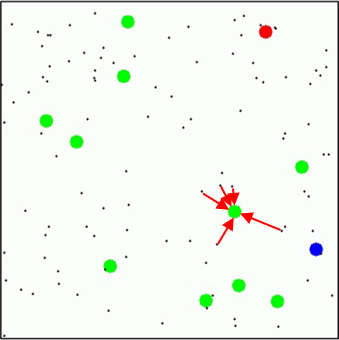
\includegraphics{bps.png}}
\caption{Continuous environment with basis points: The agent (blue) has to find the goal (red) without clliding with the obstacles (green). The red arows depict the distance to the nearest obstacle of five exemplary basis points (black).}
\label{fig1}
\end{figure}

\section{Conclusion and Outlook} 

To conclude, we have been making progress at a stable rate, advancing to the point where we were able to make an agent traverse through a continuous environment whilst avoiding multiple obstacles. From here, we plan to proceed by first perfecting our new environment representation such that no collisions occur at all. This will involve reward shaping and parameter tuning as well as trying the use of the Deep Deterministic Poliy Gradient (DDPG) algorithm instead of PPO, as that is the algorithm used in [1] very successfully. Building upon that, we hope to dynamicize the obstacles, and eventually transition from a point agent to a planar joint robot to reach the state of the art presented in [1].

\begin{thebibliography}{00}
\bibitem{b1} T. Jurgenson and A. Tamar, ``Harnessing reinforcement learning for neural
motion planning'',  \textit{arXiv preprint arXiv:1906.00214}, 2019.
\bibitem{b2} S. Prokudin, C. Lassner, and J. Romero. "Efficient learning on point clouds with Basis Point sets". \textit{Proceedings of the IEEE/CVF International Conference on Computer Vision (ICCV)}, pp. 4332–4341, 2019.

\end{thebibliography}

\end{document}
